\documentclass[a4paper, UKenglish]{article}
%% Encoding
\usepackage[utf8]{inputenx}
\usepackage[T1]{fontenc}

%% Fonts and typography
\usepackage{lmodern}           % Latin Modern Roman
\usepackage[scaled]{beramono}  % Bera Mono (Bitstream Vera Sans Mono)
\renewcommand{\sfdefault}{phv} % Helvetica
\usepackage[bf, sf]{titlesec}  % Section headings
\usepackage[final]{microtype}  % Improved typography


%% Mathematics
\usepackage{amssymb}   % Extra symbols
\usepackage{amsthm}    % Theorem-like environments
\usepackage{thmtools}  % Theorem-like environments
\usepackage{mathtools} % Fonts and environments for mathematical formuale
\usepackage{mathrsfs}  % Script font with \mathscr{}
\usepackage{amsmath}


%% Miscellanous
\usepackage{graphicx}   	% Tool for images
\usepackage{subcaption} 	% Tool for images
\usepackage[UKenglish]{babel}   % Automatic translations
\usepackage{csquotes}   	% Quotes
\usepackage{textcomp}   	% Extra symbols
\usepackage{booktabs}   	% Tool for tables
\usepackage{float}

\usepackage[usenames,dvipsnames]{xcolor}
\definecolor{lbcolor}{rgb}{0.9,0.9,0.9}
\usepackage{listings}   % Typesetting code
%\lstset{backgroundcolor=\color{lbcolor}, basicstyle = \ttfamily, frame = %single, language=python}
\lstset{
	backgroundcolor=\color{lbcolor},
	tabsize=4,
	rulecolor=,
	language=java,
        basicstyle=\scriptsize,
        upquote=true,
        aboveskip={1.5\baselineskip},
        columns=fixed,
	numbers=left,
        showstringspaces=false,
        extendedchars=true,
        breaklines=true,
        prebreak = \raisebox{0ex}[0ex][0ex]{\ensuremath{\hookleftarrow}},
        frame=single,
        showtabs=false,
        showspaces=false,
        showstringspaces=false,
        identifierstyle=\ttfamily,
        keywordstyle=\color[rgb]{0,0,1},
        commentstyle=\color[rgb]{0.133,0.545,0.133},
        stringstyle=\color[rgb]{0.627,0.126,0.941}
        }

%% Bibliography
\usepackage[backend = biber, style = alphabetic]{biblatex}
%\addbibresource{<NAME OF BIBLIOGRAPY FILE>.bib}


%% Cross references
\usepackage{varioref}
\usepackage{hyperref}
\urlstyle{sf}
\usepackage[nameinlink, capitalize, noabbrev]{cleveref}


%% Theorem-like environments
\declaretheorem[style = plain, numberwithin = section]{theorem}
\declaretheorem[style = plain,      sibling = theorem]{corollary}
\declaretheorem[style = plain,      sibling = theorem]{lemma}
\declaretheorem[style = plain,      sibling = theorem]{proposition}
\declaretheorem[style = definition, sibling = theorem]{definition}
\declaretheorem[style = definition, sibling = theorem]{example}
\declaretheorem[style = remark,    numbered = no]{remark}


%% Delimiters
\DeclarePairedDelimiter{\p}{\lparen}{\rparen}   % Parenthesis
\DeclarePairedDelimiter{\set}{\lbrace}{\rbrace} % Set
\DeclarePairedDelimiter{\abs}{\lvert}{\rvert}   % Absolute value
\DeclarePairedDelimiter{\norm}{\lVert}{\rVert}  % Norm


%% Operators
\DeclareMathOperator{\im}{im}
\DeclareMathOperator{\rank}{rank}
\DeclareMathOperator{\E}{E}
\DeclareMathOperator{\Var}{Var}
\DeclareMathOperator{\Cov}{Cov}


%% New commands for sets
\newcommand{\N}{\mathbb{N}}   % Natural numbers
\newcommand{\Z}{\mathbb{Z}}   % Integers
\newcommand{\Q}{\mathbb{Q}}   % Rational numbers
\newcommand{\R}{\mathbb{R}}   % Real numbers
\newcommand{\C}{\mathbb{C}}   % Complex numbers
\newcommand{\A}{\mathbb{A}}   % Affine space
\renewcommand{\P}{\mathbb{P}} % Projective space


%% New commands for vectors
\renewcommand{\a}{\mathbf{a}}
\renewcommand{\b}{\mathbf{b}}
\renewcommand{\c}{\mathbf{c}}
\renewcommand{\v}{\mathbf{v}}
\newcommand{\w}{\mathbf{w}}
\newcommand{\x}{\mathbf{x}}
\newcommand{\y}{\mathbf{y}}
\newcommand{\z}{\mathbf{z}}
\newcommand{\0}{\mathbf{0}}
\newcommand{\1}{\mathbf{1}}


%% Miscellanous
\renewcommand{\qedsymbol}{\(\blacksquare\)}


%% Things I've put in meself
\usepackage{tikz}
\usetikzlibrary{decorations.pathreplacing,angles,quotes}
\newcommand*\circled[1]{\tikz[baseline=(char.base)]{
            \node[shape=circle,draw,inner sep=2pt] (char) {#1};}}
\usepackage{arydshln}



\begin{document}
\title{FYS-STK 3155 project 2}
\author{Theodor Midtbø Alstad}
\maketitle

\begin{abstract}
This report compares a neural network to numerical stochastic gradient descent linear regression, analytical Ridge linear regression, and logistic regression for classification. It finds that the neural network outperforms all compared methods for linear regression, and is outperformed by the logistic regression for classification because it had more features implemented.
\end{abstract}

\section{Introduction}
[Start the introduction with a motivation of the topic, then move on to a discussion of the structure of the report.]

A neural network is a very flexible data analysis tool that can grant a large amount of knowledge about correlations between features when applied to a large enough volume of data, but it requires a lot of optimization and parametrization. It is therefore important to ascertain that it does perform well enough to be worth the time and resources building and training it takes.

In this project, I first implement and study Stochastic Gradient Descent where I compare it as a simple numerical approach with analytical approaches in OLS and Ridge and use them as a basis to determine how well the neural network performs linear regression. I implement and study a logistic regressor as a basis to determine how well the neural network performs classification. Finally, I implement and study a Neural Network as the most detailedly implemented algorithm, and studied determined whether it outperformed the previously mentioned algorithms for linear regression and classification.

This report contains a regression analysis on the Franke function (\autoref{sec:Franke}) and a classification analysis on the MNIST dataset (\autoref{sec:MNIST}) as a basis for evaluating the Neural Network.


The scripts for the Stochastic Gradient Descent and Linear Regression are not optimized for user friendliness, as the were created to form a basis for comparison for the neural network.

\subsection{The structure of the source code and filesystem}
The source code is split into 3 main scripts and 3 side scripts.

Main scripts:
\begin{itemize}
\item SGD.py: Stochastic Gradient Descent algorithm; regresses. Imports from miscFunctions.py, handles its own data.
\item NeuralNetwork.py: Neural network; regresses and classifies. Imports from miscFunctions.py, activationFunctins.py, and dataHandler.py, has its data handled by dataHandler.py
\item LogisticRegression.py: Logistic Regression algorithm; classifies. Imports from activationFunctions.py and miscFunctions.py, handles its own data.
\end{itemize}

Side scripts:
\begin{itemize}
\item dataHandler: Loads, generates, and handles datasets as well as handles plotting for NeuralNetwork.py, 
\item miscFunctions.py: Contains functions needed for functionality such as to\_categorical\_numpy, which transforms arrays into one-hot form, or defaulting func, which selects default values according to a priority list.
\item activationFunctions.py: Contains activation functions, such as softMax or ReLU\_leaky for use in logistic regression and the Neural Network.
\end{itemize}

Tested parameters are stored in the folder parameterValues. Analysis of the parameters is stored in text-form in LaTeX/appendix/analyzedParameters and in imageform in LaTeX/images. Source code files are stored directly in the main folder.


\subsection{Franke function} \label{sec:Franke}
The Franke function is the model used for linear regression. It is here defined for the domain $x,y \in [0,1]$
\begin{align*}
f(x,y) &= \frac{3}{4}\exp{\left(-\frac{(9x-2)^2}{4} - \frac{(9y-2)^2}{4}\right)}+\frac{3}{4}\exp{\left(-\frac{(9x+1)^2}{49}- \frac{(9y+1)}{10}\right)} \\
&+\frac{1}{2}\exp{\left(-\frac{(9x-7)^2}{4} - \frac{(9y-3)^2}{4}\right)} -\frac{1}{5}\exp{\left(-(9x-4)^2 - (9y-7)^2\right) }
\end{align*}


\subsection{MNIST dataset} \label{sec:MNIST}
For classification methods, I use the MNIST image dataset. It contains 1797 entries of low-resolution images of the numbers 0-9 and accompanying labels describing what number the image portrays. there are 178 entries labelled 0 out of 1797 entries, making up 9.905\% of the dataset, meaning any method that has a 9.905\% accuracy is likely to have overflown weights and is predicting every label to be 0.

\subsection{Ordinary Least Squares (OLS) and Ridge}
The OLS and Ridge methods, used in this project as comparison points for the linear regression, attempt to model a dataset by minimizing the square error between the dataset, $z$, and a model in the form $\hat{z} = \textbf{X}\theta$, where $\textbf{X}$ is a design matrix and $\theta$ is a vector of parameters.

OLS analytically minimizes the cost function $C = \mathbb{E}[(z - \hat{z})^2]$ by using parameters $$\theta = \left(\textbf{X}^T\textbf{X}\right)^{-1} \textbf{X}^T y $$

Ridge amends OLS, attempting to mitigate issues brought by uninvertible or near-uninvertible design matrices, by adding a diagonal value before the inversion: $$\beta = \left(\textbf{X}^T\textbf{X} + \lambda \textbf{I}\right)^{-1} \textbf{X}^T y $$
\subsection{Stochastic Gradient Descent (SGD)}
Stochastic Gradient Descent revolves around making prediction from a design matrix, initialized in some pre-determined way (here as random noise), $X$, to an expected value, $z$, with a 1D array, $\theta$, finding an error, and adjusting the array $\theta$ with a gradient based on that error. The idea is that $\theta$ will follow a gradient in the error-parameter space towards a location of an error minimum.

SGD as a method will attempt to regress and interpolate between datapoints to approach a continuous function.

The cost function used in this report for optimization is the MSE: $C(\theta) = \frac{1}{n}(\textbf{X}\theta - z)^T(\textbf{X}\theta - z)$. The gradient is hence given as $\nabla C(\theta) = 2\textbf{X}^T((\textbf{X}\theta) - z)$


\subsubsection{Momentum}
An option for optimizing the gradient descent is to implement a momentum feature. It functions as a running average with linearly increasing weights. Every iteration reduces the momentum by a factor and adds the current gradient to it; $\text{momentum} \leftarrow \text{momentum}\times \rho + \nabla C(\theta) $, where $0 \leq \rho \leq 1$ is a drag factor 

\subsubsection{Minibatching}
When optimizing on a gradient, there is no guarantee that there is only one minimum within the cost-space, and it is possible to be caught in local minima that have a larger error than the global minimum that we are searching for. To solve this, one could force more noise onto the gradient by adjusting for only one datapoint at a time, but this is very inefficient and removes parallelized computation as a possibility. In this project, minibatching is used to compromise between these. Minibatching calculates a gradient for a number of randomly selected points, making entrapment in local less likely while still maintaining efficiency. The cost function gradient can then be described as a sum of these points: $\nabla C(\theta) = \sum\limits_{k} \nabla_\theta c_k(\textbf{x}_k,\theta)$, where $k$ is a subset of the original points referred to as the minibatch; $k\in K \in N$.

\subsubsection{Varying step length} \label{sec:varying step length}
Step length is a factor multiplied onto the gradient that is applied to the weights in a descent-based method as a regularization tool. If the step-length is too small, the solution might be stuck in local minima or not find a solution in time. If the step length is too large, the solution might diverge. A varying step length can be implemented to move out of local minimum but still find accuracy within the minimum at the end of the training process. In this project, this is implemented as $\eta = \frac{t_1}{t + t_0}$ where $\eta$ is the step length, $t_0$ and $t_1$ are parameters to be adjusted, and t is an incrementing integer, starting at 0 and incrementing on each call.


\subsection{Logistic Regression}
Following a similar concept to SGD, logistic regression attempts to approximate a discrete dataset, typically being used as a classification tool. Where linear SGD will estimate the heigh of an entity, a logistic regressor will estimate whether that entity is a hill or a building. 

In the instance of this project, the distinct classes are split into one-hot vector form and put through the Softmax function to determine what class has the best fit.

A logistic regression algorithm comes here in the form of $(\text{prediction} = f(\textbf{X}\theta))$, $(\text{error} = \text{prediction} - z)$, and $(\theta \leftarrow \theta - X^T \text{error}) $ where $f()$ is the activation function, here Softmax.


\subsubsection{$l_2$ regularization parameter}
In order for weights not to diverge to overflow, regularization may be implemented in addition to the step length. $l_2$ regularization refers to having an $l_2$-parameter between 0 and 1 that is multiplied by the sum of the squares of the weights to get an $l_2$-term, which is then added to the gradient. Since the gradient is subtracted from the weights, this can keep the weights from diverging.


\subsection{Neural Network}
An extension to logistic regression, a neural network places multiple layers between the input and the output, where each layer is considered an input to the following and output to the prior layer, allowing for modelling of much more complex problems.

\section{Method}
There are four methods tested, SGD, Ridge, Neural Network, and Logistic Regression. They have all been optimized by being given a parameter space, a combination of multiple parameters, having their accuracy tested on all of them, and selecting the best one. Further analysis is done on the parameters of this parameter-space.

\subsection{SGD} 
To evaluate SGD, I implemented an SGD-algorithm with momentum, which was compared to analytical solutions Ordinary Least Squares (OLS) and Ridge. The algorithm was applied to a generated dataset made of a two-dimensional polynomial where both dimensions, $x$ and $y$, where $x, y \in [0,1]$. The polynomial was compared to the Franke function of those $x$- and $y$-values.

I then ran it through the all combinations of a set of parameters as given in the list below and found the optimal combination, and used those parameters to plot $R^2$ and MSE as a function of the number of epochs.

The SGD data values were not split into training and testing sets, unlike the NN data, due to time constraints.

Parameters adjusted:
\begin{itemize}
\item Number of Datapoints in the dataset: 50, 100
\item Polynomial degree of the dataset: 5, 8, 10, 12, 15
\item Size of the minibatches: 10, 50, 100
\item Number of epochs: 250, 500
\item Different combinations of $t_0$ and $t_1$: (10, 10), (10, 50), (10, 1)
\item Momentum coefficient: 0.00, 0.25, 0.50, 0.75, 1.00
\end{itemize}

Finally, I looked at Ridge as a function of the $\lambda$-parameter to compare to my SGD solution.

\subsection{Logistic Regression}
To evaluate Logistic Regression, I implemented a logistic regression algorithm using momentum and an $l_2$-term. These values where evaluated against the accuracy of neural network that also was developed (\autoref{sec:NN method}.

Similarly to the SGD-algorithm, the logistic regression-algorithm was tested through the parameter space, and the optimal set of parameters was selected from this.

The logistic regression data values were not split into training and testing sets, unlike the NN data, due to time constraints.

Parameters adjusted:
\begin{itemize}
\item Different combinations of $t_0$ and $t_1$: (1, 1), (1, 3.16), (1, 10), (1, 31.6), (1,100)
\item Number of epochs: 50, 100, 500, 1000
\item Size of the minibatches: 16, 32, 64, 128
\item Momentum coefficients: 0.0, 0.1, 0.2, 0.3, 0.4, 0.5, 0.6, 0.7, 0.8, 0.9, 1.0
\item $l_2$ parameters: 10, 1, 0.1, 0.01, 0.001, 0.0
\end{itemize}

I then analyzed the accuracy score of the logistic regression as a function of the $l_2$-parameter and $\eta$.

\subsection{Neural Network} \label{sec:NN method}
The neural network was made before the logistic regressor, and the regressor was treated as a special case of a neural network, where there were 0 hidden layers. Since the neural network can both linearly regress and classify, it was compared to both SGD and logistic regression, spending 33 hours calculating the optimal paremeters for the linear regression and 23 on the classification parameters. Since this is the main focus of the project, more time was spent analyzing the parameterspace for the NN than for the SGD-algorithm or the logistic regressor.

The biases were initialized at 0.01 and the weights were initialized as randomly distributed with a mean of 0 and a standard deviation of 1.

The softmax function was selected as output function for classification due to its normalization of the values given. For the linear regression, a linear function with a single parameter, $\alpha$, was used as a coefficient for the output. A linear function was chosen because a linear output can very easily approximate a linear function.

First I generated each combination of the parameters set and calculated an associated score as an average over 5 runs for each combination of the parameters. This was stored in a file. I then analyzed the score as a function of the $\lambda$-parameter and the $\eta$-parameter, with $\eta$ as both a constant and as a decreasing value (\autoref{sec:varying step length}). I then compared the different activation functions to eachother.

Finally, I compared the performance of the neural network as a linear regressor to the performance of the SGD algorithm and Ridge and its performance as a classifier to the performance of the logistic regressor (\autoref{sec:algorithm-comparison}).

Parameters adjusted for linear regression:
\begin{itemize}
\item Number of hidden layers: 0, 1, 2, 4
\item Number of nodes: 16, 32, 48, 64
\item Number of epochs: 250, 500
\item Size of minibatch: 32, 64
\item $\eta$, as $t_0/(t+t_1)$: (1, 1), (1, 10), (1, 100), (1, 1000), (1, 10000),  (1, 100000), (1, 1000000)
\item $\eta$, as a constant: 1, 0.1, 0.01, 0.001, 0.0001, 0.00001, 0.000001
\item $\lambda$: 0.1, 0.01, 0.001, 0.0001, 0.00001, 0.000001
\item $\alpha$: 0.1, 0.01, 0.001
\item Activation function for the hidden layers: sigmoid, ReLU\_leaky, ReLU
\item Activation function for the output layer: softmax
\end{itemize}

Parameters adjusted of classification:
\begin{itemize}
\item Number of hidden layers: 0, 1, 2
\item Number of nodes: 16, 32
\item Number of epochs: 250, 500, 750
\item Size of minibatch: 32, 64, 128
\item $\eta$, as $t_0/(t+t_1)$: (1, 1), (1, 10), (1, 100), (1, 1000), (1, 10000),  (1, 100000), (1, 1000000)
\item $\eta$, as a constant: 1, 0.1, 0.01, 0.001, 0.0001, 0.00001, 0.000001
\item $\lambda$: 0.1, , 0.00316, 0.000001
\item $\alpha$: 1, 0.1
\item Activation function for the hidden layers: sigmoid, ReLU\_leaky, ReLU
\item Activation function for the output layer: softmax
\end{itemize}


For the neural network, the data is split into training and test data (75/25 split), where the data is trained on the training data and tested on the test data. This prevents overfitted functions from receiving too high a score.

\section{Results/Discussion}


\subsection{SGD} 
\begin{figure}[H]
        \centering 
        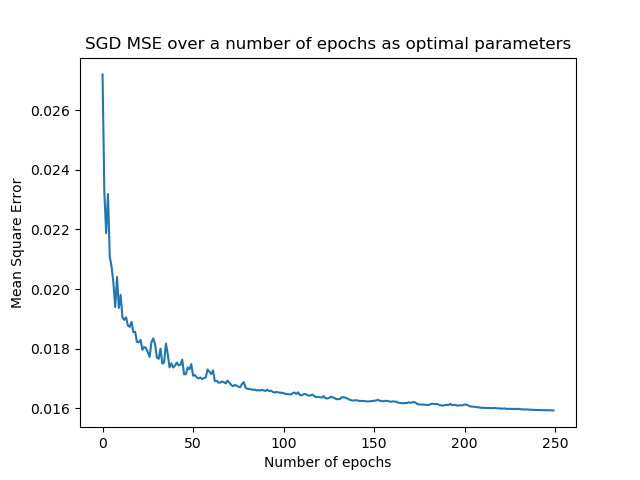
\includegraphics[scale=0.7]{images/partA_MSE.png} 
        \caption{Shows how well the SGD solution approaches the Frankefunction as a function of the number of epochs by using the MSE of the training data.}
        \label{fig:partA_MSE}
\end{figure}


\begin{figure}[H]
        \centering 
        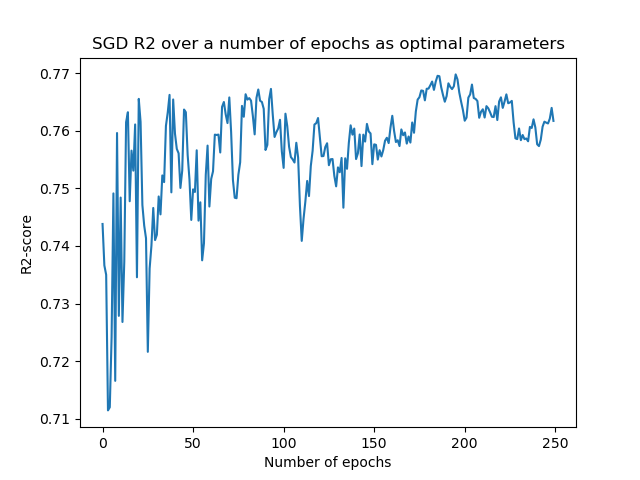
\includegraphics[scale=0.7]{images/partA_R2.png} 
        \caption{Shows how well the SGD solution approaches the Frankefunction as a function of the number of epochs by using the $R^2$-score of the training data.}
        \label{fig:partA_R2}
\end{figure}


\begin{figure}[H]
        \centering 
        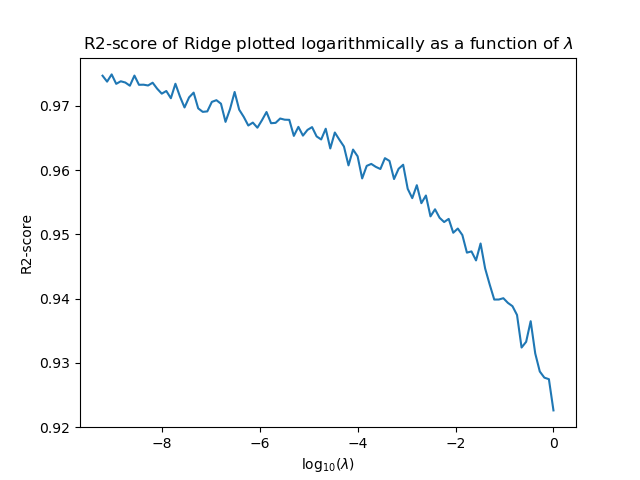
\includegraphics[scale=0.7]{images/partA_ridge.png} 
        \caption{Shows how well the ridge solution approaches the Frankefunction as a function of the $\lambda$-parameter by using the $R^2$-score.}
        \label{fig:partA_ridge}
\end{figure}

\autoref{fig:partA_MSE} and \autoref{fig:partA_R2} show that, perhaps unsuprisingly, a greater number of epochs leads to a higher accuracy, although the $R^2$ seems to vary a large amount. This is perhaps due to the cost function being based on the MSE and not the $R^2$.

The fact that this is all training data and not test data suggests that the MSE and $R^2$ should not be trusted too highly at a higher number of epochs.



\begin{table}[H] 
\centering
\caption{A sample of $\lambda$-values with an associated $R^2$ score.}
\label{tab:Ridge performance}
\begin{tabular}{|c|c|}
  \hline
  $\lambda$ & $R^2$ \\
  \hline
  1.0 & 0.922590 \\
  0.117681 & 0.952397 \\
  0.0001 & 0.974680 \\
  0.0/OLS & 0.979087 \\
  \hline
\end{tabular}
\end{table}


The analytical Ridge-solution reaches much higher $R^2$-scores than the numeric SGD, suggesting that a simple numeric approach is not good enough to model the Franke function. The analytical solution performs best as a standard OLS, or with $\lambda = 0$.

\begin{table}[H] 
\centering
\caption{Shows score reached as a function of $\eta$. An $\eta$-value containing a "None" means that the other value is considered as a constant eta value.}
\label{tab:SGD eta-values}
\begin{tabular}{|c|c|c|c|c|}
	\hline
Eta-values & Average $R^2$ & Median $R^2$ & Maximum $R^2$ & Non-overflown SGD's [\%]\\
\hline
('10', '10')       & 0.688806 & 0.742613 & 0.797290 & 1.0 \\
('10', '1')        & 0.620894 & 0.759868 & 0.793156 & 1.0 \\
('10', '50')       & 0.680007 & 0.737220 & 0.799657 & 1.0 \\
('100', '1')       &-0.007316 &-0.001517 &-6.968662e-08 & 0.9375 \\
('50', '1')        &-0.005946 &-0.000307 &-4.494689e-10 & 0.979167 \\
('None', '0.1')    & 0.820982 & 0.874075 & 0.925629 & 0.943333 \\
('None', '0.01')   & 0.786223 & 0.736666 & 0.884543 & 1.0 \\
('None', '0.001')  & 0.646276 & 0.810326 & 0.844811 & 1.0 \\
	\hline
\end{tabular}
\end{table}

\begin{table}[H] 
\centering
\caption{Optimal values found with associated $r^2$ score. Franke was generated with 200 points on each axis, and a design matrix of polynomial degree 15 was used.}
\label{tab:SGD optimal values}
\begin{tabular}{|c|c|c|c|c|}
	\hline
  $R^2$ & (t0, t1) & \# of epochs & Minibatch size & Momentum-coefficient \\
  \hline
  0.760531 & (10, 1) & 1000 & 128 & 0.0 \\
	\hline
\end{tabular}
\end{table}

\autoref{tab:SGD eta-values} seems to strongly favour constant $\eta$-values, as is also reflected in \autoref{sec:NN results}. This is unexpected and may be due to poorly chosen $t_0$ and $t_1$ values, but due to constant values performing better for every value, this seems unlikely.

\subsection{Logistic Regression}
\begin{figure}[H]
        \centering 
        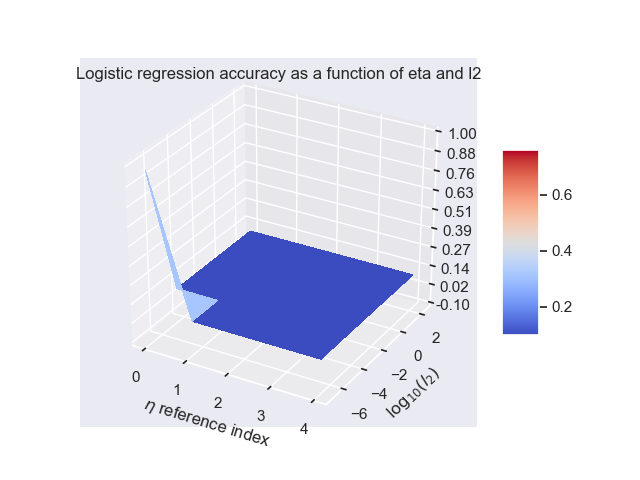
\includegraphics[scale=0.7]{images/partE_l2andeta.png} 
        \caption{shows how well the logistic regression predicts the correct labels as a function of the $l_2$- and $\eta$-parameter. The $\eta$-reference index refers to $t_0 \text{ and } t_1$ in order as (1.0, 100.0), (1.0, 31.622777), (1.0, 10.0), (1.0, 3.162278), (1.0, 1.0).}
        \label{fig:partE_l2andeta}
\end{figure}


\begin{table}[H] 
\centering
\caption{Optimal values found with associated accuracy score.}
\label{tab:LogReg optimal values}
\begin{tabular}{|c|c|c|c|c|c|}
	\hline
  Accuracy & (t0, t1) & \# of epochs & Minibatch size & Momentum-coefficient & l2
  \\
  \hline
  0.987201 & (1, 31.622777) & 1000 & 128 & 0.9 & 0.0 \\
	\hline
\end{tabular}
\end{table}



\autoref{fig:partE_l2andeta} reflects a poor choice in $\eta$ and $l_2$ values, as most of the graph shows an accuracy of 9.905\% which implies, as mentioned in \autoref{sec:MNIST}, that the weights overflowed. \autoref{tab:SGD eta-values} shows an error rate of 1.28\%, which is a fairly high performance when compared to the values found at [1]



\subsection{Neural Network} \label{sec:NN results}
\begin{table}[H] 
\centering
\caption{$R^2$ score reached for each activation function}
\label{tab:activation functions}
\begin{tabular}{|c|c|c|c|c|c|}
  \hline
  Function & Average & Median & Maximum & Non-overflown NN's [\%] \\
  \hline
  ReLU\_leaky &-37160.106071 & -1.620086 & 0.900225 & 0.982143 \\
  ReLU        &-43070.479707 & -1.975616 & 0.863374 & 0.982143 \\
  sigmoid     &-5.518974+194 & -1.202853 & 0.882485 & 0.943204 \\
  \hline
\end{tabular}
\end{table}


\begin{figure}[H]
        \centering 
        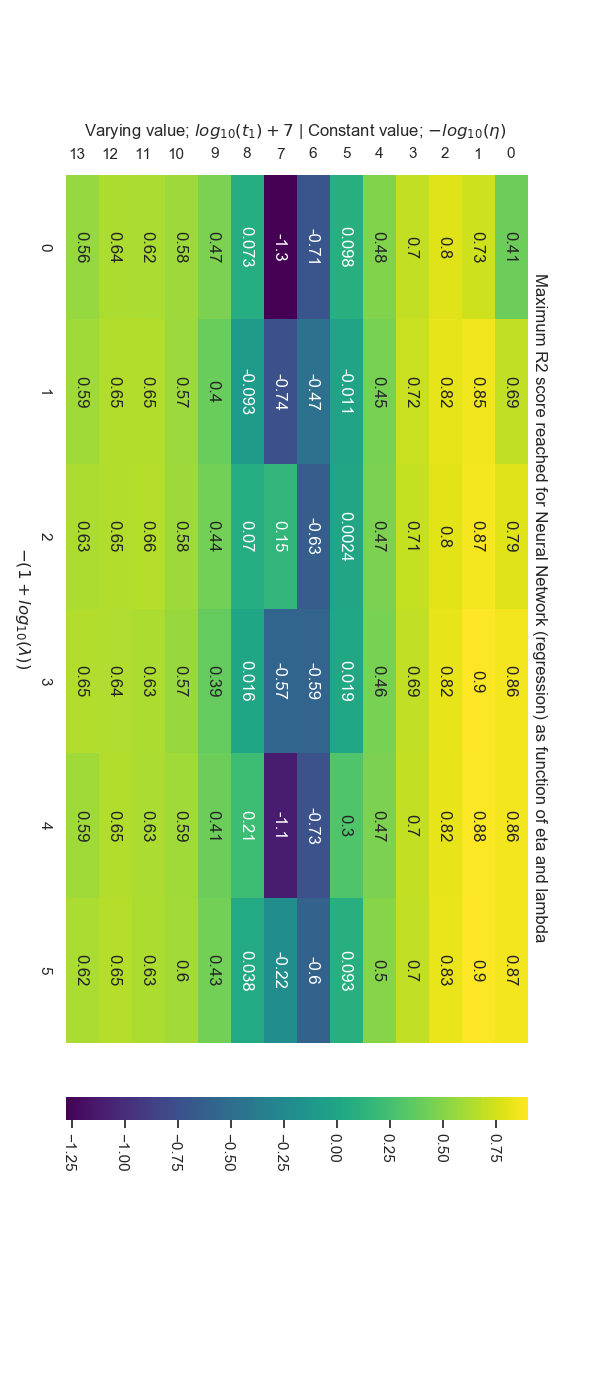
\includegraphics[scale=0.6]{images/partB.png} 
        \caption{$R^2$ score as a function of $\eta$ and $\lambda$. The axes are numbered by indexes, not actual axis value, but axis labels describe the conversion between the values and the indexes. The $\eta$-axis is split into constant $\eta$, indices 0 to 6 inclusive, and varying $\eta$, indices 7 to 13 inclusive. Varying $\eta$ assumes $\eta = t_0/(t+t_1)$ where $t_0=1$}
        \label{fig:covers the page}
\end{figure}

From \autoref{tab:activation functions}, ReLU\_leaky managges to outperform both ReLU and sigmoid in nearly every aspect (scoring equally well to ReLU in number of overflown NN's), and was found to be the optimal activation function for both classification and linear regression. Meanwhile, whilst sigmoid outperformed ReLU at its best and at its median, it overflowed more networks, and thus seems less stable or reliable.

From \autoref{fig:covers the page}, a constant $\eta$ performs better than a varying $\eta = t_1/(t+t_0)$, optimally at $\eta = 0.1$, paired with $\lambda = 1e-4 \text{ or } 1e-6$.

\begin{table}[H] 
\centering
\caption{Optimal parameters with an increased number of epochs. The classification network was trained for 1000 epochs with a minibatch of 32 datapoints, while the linear regression network was trained for 5000 epochs with a minibatch of 32 datapoints.}
\label{tab:optimal NN}
\begin{tabular}{|c|c|c|c|c|c|c|c|c|}
  \hline
  Mode & Score & Layers & Nodes & $(t_0, t_1)$ & $\lambda$ & $\alpha$ & activFunc & outFunc\\
  \hline
  Classification & 0.971 & 0 & 32 & (1, 1e3) & 0.1 & 1.0 & ReLU\_leaky & softmax \\
  \hline
  Linear regression & 0.994 & 1 & 32 & 0.1 & 1e-4 & 0.1 & ReLU\_leaky & linearActivation \\
  \hline
\end{tabular}
\end{table}



\subsection{Comparing the algorithms} \label{sec:algorithm-comparison}
\subsubsection{Regression}
The neural network manages to attain an $R^2$ score of 0.994 (\autoref{tab:optimal NN}) compared to SGD's 0.760 (\autoref{tab:SGD optimal values}) and OLS' 0.979 (\autoref{tab:Ridge performance}). This makes a neural network a much stronger tool for linear regression than basic SGD for the Franke function, and outperforms analytical Ridge and OLS. This should be contrasted with the difficulty of implementation and optimization, where OLS is very easy to implement and takes no resources to optimize (just training), compared to the slightly harder SGD and much harder NN.

\subsubsection{Classification}
The neural network manages to attain an accuracy score of 0.971 (\autoref{tab:optimal NN}), compared to the logistic regressions 0.987 (\autoref{tab:LogReg optimal values}), indicating that a simple logistic regression outperforms a neural network, even when that network has 0 layers, emulating a simple logistic regression algorithm. Since the optimal logistic regression $l_2$-parameter was found to be 0, this is likely to be due to the momentum feature implemented into the logistic regression, having a momentum-coefficient of 0.9. I expect that if the $l_2$-parameter and the momentum-feature were to be implemented into the neural network, it would not be outperformed by the logistic regression algorithm, as it should be able to emulate its performance with 0 hidden layers.

\subsection{Improvements}
In this project I have exclusively used the MNIST dataset and the Franke function, and I would be able to get a stronger basis for any conclusions if I spread the analysis over more datasets or functions.


\section{Conclusion}
The neural network outperforms all other tried methods (SGD, Ridge, and OLS) for linear regression based on $R^2$-score. The neural network is outperformed by a logistic regression-algorithm when used for classification, but this is assumed to be due to additional features being implemented into the logistic regression (momentum and $l_2$-regularization), as a neural network should be able to emulate a logistic regression by using 0 hidden layers. The expectation is that if those features were to be implemented into the neural network, it would be able to outperform all other methods tested.

\section{References}
[Check out how to refer to web pages. A single URL is not enough.]
\begin{itemize}
\item [1] Y. LeCun, L. Bottou, Y. Bengio and P. Haffner: \textit{Gradient-Based Learning Applied to Document Recognition}, Proceedings of the IEEE, 86(11):2278-2324, November 1998, retrieved from http://yann.lecun.com/exdb/mnist/
\end{itemize}


\section{Appendix}


\end{document}